\subsubsection{Procedure}
Each participant was tested individually in a small meeting room (see Figure \ref{fig:test_setup}). Besides the participant, a facilitator and an observer was also present in the room. The participant were given a brief introduction and was subsequently presented with a consent form. With their consent, the test began and video recording started. The participants started by answering a demographic questionnaire on a laptop. After this they were introduced to a demo of the Camera Path Animator (see Section \ref{relatedWork}). This was to give the participant context for the test and to introduce them to the concept of camera behaviour in an interactive environment. 

\begin{figure}[htbp]
\centering
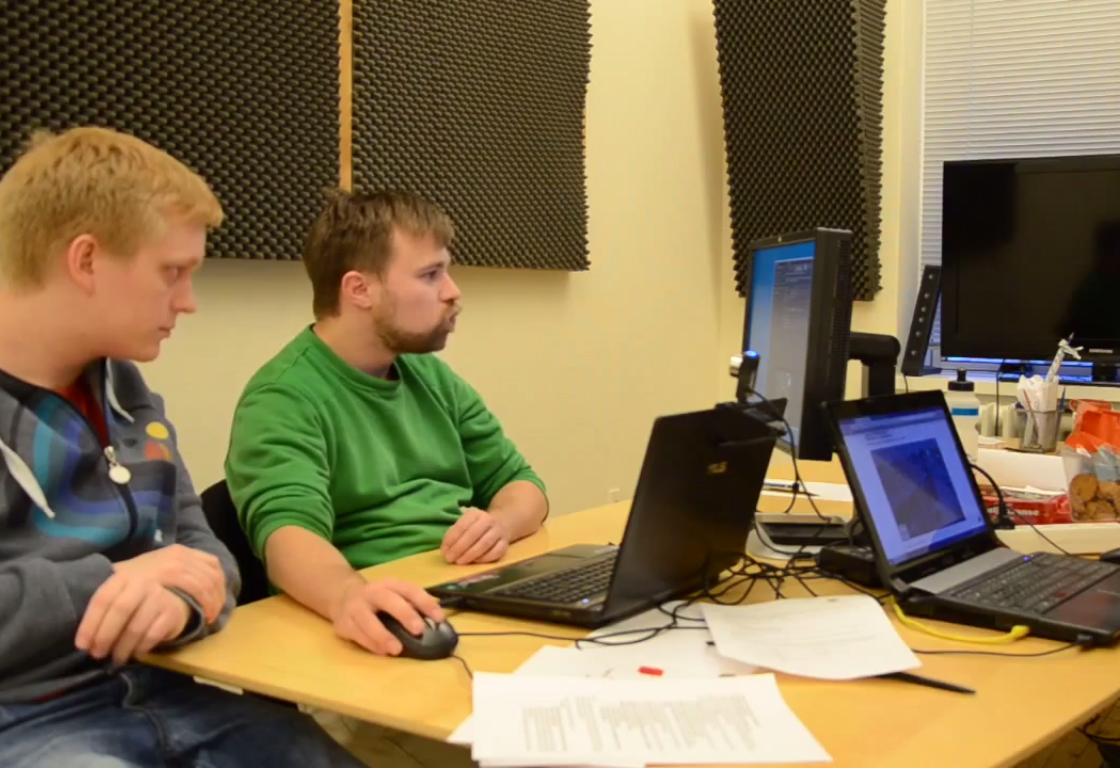
\includegraphics[width=0.3\textwidth]{Pics/test_setup}
\caption{The test participant used had two monitors at his disposal while working with the tool.}
\label{fig:framingConcept}
\end{figure}

The participants and facilitator sat down at another laptop with a second monitor connected. Here the facilitator gave the participant a basic introduction to Unity to ensure that all participants had no problem of navigating and manipulating the workspace. The participant was tasked to move the camera to three specific locations in the environment to ensure they felt comfortable in the workspace. \textbf{Training:} After this the facilitator introduced the camera tool to the participant, first he explained the concept with pen and paper, then he opened the tool in Unity and explained its features and functionalities. The participant was asked to try each feature as they were introduced, e.g. when the facilitator explained how to place influence points and how to connect them, the participant was asked to try it for themselves. \textbf{Tasks:} When all features were explained, and the facilitator felt that the participant had a \textbf{good grasp (!!!)} on the tool, the participant was handed a piece of paper with 5 tasks such as \textit{"Make the camera's field of view change"} and \textit{"Make the camera go from a low perspective to bird's eye view."} listed on it. The participant had to solve the tasks themselves, the facilitator only intervened when the participant was struggling with something, asked a question, or at unforeseen occurrences (e.g. bugs). \textbf{Creative:} After this, the participant was introduced to a level with a modelled environment. They were then tasked to envision and sketch two ways for the camera to move as the play character moved through this environment, when they had two ideas, they were tasked to implement both of these using our camera tool. The facilitator remained as neutral as possible for this part of the test, but still intervened if they participant was struggling or encountered things like bugs.

Finally, the participant went back to the first laptop and answered a post-test questionnaire. The participant was thanked and the test ended.